\documentclass[%
 reprint,
 %superscriptaddress,
 %groupedaddress,
 %unsortedaddress,
 %runinaddress,
 %frontmatterverbose,
 %preprint,
 showpacs,
 showkeys,
 preprintnumbers,
 %nofootinbib,
 %nobibnotes,
 %bibnotes,
 amsmath,amssymb,
 aps,
 % prl,
 pra,
 % prb,
 % rmp,
 %prstab,
 %prstper,
  longbibliography,
 %floatfix,
 %lengthcheck,%
 ]{revtex4-1}

\usepackage[breaklinks=true,colorlinks=true,anchorcolor=blue,citecolor=blue,filecolor=blue,menucolor=blue,pagecolor=blue,urlcolor=blue,linkcolor=blue]{hyperref}
\usepackage{graphicx}% Include figure files
\usepackage{xcolor}

\usepackage{amsthm}
\usepackage{bbm}
\usepackage{graphicx}
%\usepackage{ifsym}
\usepackage{MnSymbol}

\newtheorem{prop}{Proposition}
\newtheorem{theorem}{Theorem}
\newtheorem{lemma}{Lemma}
\newtheorem{cor}{Corollary}
\theoremstyle{definition}
\newtheorem{defn}{Definition}


 \begin{document}
\sloppy



\title{Zeno Squeezing of Cellular Automata}

\author{Martin Schaller}
\affiliation{Algorithmics, Parkring 10, A-1010  Vienna, Austria}
\email{martin\_schaller@acm.org}

\author{Karl Svozil}
\affiliation{Institute of Theoretical Physics, Vienna
    University of Technology, Wiedner Hauptstra\ss e 8-10/136, A-1040 Vienna, Austria}
\email{svozil@tuwien.ac.at} \homepage[]{http://tph.tuwien.ac.at/~svozil}


\date{\today}

\begin{abstract}
We have recently introduced two new models of computations: self-similar cellular automata and self-similar Petri nets.
Self-similar automata result from a progressive, infinite tessellation of space and time.
Self-similar Petri nets consist of a potentially infinite sequence of coupled transitions with ever
increasing firing rates.
Both models are capable of hypercomputations and can, for instance, ``solve'' the halting problem for Turing machines.
We survey the main theory, state a new proposition about the indeterminism of self-similar cellular automata and
present a simplified construction of a hypercomputer within self-similar cellular automata.
\end{abstract}

\pacs{02.70.-c, 02.10.Ox}
\keywords{Zeno squeezing, cellular automata, hypercomputation}
\maketitle



\section{Introduction}

Self-similar cellular automata are closely related to cellular automata, a class of dynamical systems
characterized by discreteness in space, time, state values, determinism,
and local interaction (see e.g.,~\cite{gutowitz91}).
A cellular automaton is an infinite lattice of finite automata, each linked with its neighboring automata,
whose underlying space-time structure results from a uniform tessellation of space and time.
In contrast, the underlying space-time structure of a self-similar automaton
is based on a progressive tessellation of space and time, the very same tessellation
that Zeno considered in his paradox of the runner that cannot reach the end of a racecourse
(see e.g.,~\cite{salmon-01}).
Whereas all cells in a one-dimensional cellular automaton are updated synchronously, a cell in
a self-similar cellular automaton is updated twice as often as its left neighbor.
On the one hand, this modification results in completely new capabilities; for instance, there exist
self-similar cellular automata that are capable of hypercomputing.
On the other hand, new paradoxes arise; for instance, the evolution of a self-similar
cellular automaton that involves an infinite number of steps might lead to a form of
indeterminism that relates to Thomson's lamp paradox \cite{thom:54}.

The carry-over of the self-similar cellular automaton model to the theory of Petri nets
(see, e.g.,~\cite{Murata89}) yields self-similar Petri nets.
They are equivalent to self-similar cellular automata for a finite number of calculation steps, but differ in the infinite case.
Self-similar Petri nets avoid the indeterminism of self-similar cellular automata by
halting in the infinite case.

As already mentioned, both self-similar cellular automata as well as self-similar Petri nets have been introduced in \cite{2008-sica}.
There are several aspects that make both
models  interesting.
Both can be seen as variations of Zeno's original paradox, leading to new classes of supertasks (see e.g.,~\cite{en96})
and both allow the construction of hypercomputers,
and thus demonstrating that it is possible to build hypercomputers based
on simple building blocks: either finite automata or Petri net transitions.
Since the two models differ operationally only in the infinite limit,
new questions about causality and the ontological structure of space and time arise.

The physical plausibility of accelerating Turing machines, supertasks, and Zeno-like processes,
is discussed elsewhere (see, e.g.,~\cite{sv-aut-rev}).
Originally conceived as a means to demonstrate self-reproduction capabilities in a universal computing
environment by von Neumann~\cite{v-neumann-66},
the idea of perceiving the physical universe as cellular automaton goes back to Zuse \cite{zuse-67} and was
developed further  by other researchers~\cite{fredkin,toffoli-margolus-90,wolfram-2002}.
Cellular automata based on other tessellations than the uniform grid  were studied in~\cite{margenstern99}.
Hypercomputing is a fast-growing field (see, e.g.,~\cite{ord-2006, stannett06}),
despite criticism related to the methodology and the classification of
 what should be considered a valid computing process ~\cite{Davis-2004,Davis-2006,potgieter-06}.

For other approaches that use the infinite divisibility of Newtonian space-time to construct hypercomputers
see \cite{beggs-tucker-06,Davies01,svozil-2007-cestial}.
Another more abstract approach is described in ~\cite{durand-lose09} that investigates abstract
geometrical computations that naturally arise as a continuous
counterpart of cellular automata.

The article is organized as follows.
Section \ref{sec:ssca} defines self-similar cellular automata, presents the basic properties and states a new
proposition about the indeterminism of self-similar cellular automata.
Section \ref{sec:hypercomputer} gives a new construction of a hypercomputer
that simplifies the construction presented in \cite{2008-sica}.
Self-similar Petri nets are surveyed in Section \ref{sec:petri}.
The final section contains some concluding remarks and gives some directions for future research.

\section{Self-Similar Cellular Automata}
\label{sec:ssca}

\subsection{Basic Definitions}

The underlying structure of a cellular automaton results from a uniform tessellation of space and time.
Figure \ref{fig:ca-evo} depicts the evolution of a cellular automaton.
In contrast, self-similar automata result from a progressive tessellation of space and time.
A self-similar cellular automaton operates as a cellular automaton on a one-dimensional lattice containing an infinite number of cells.
Moreover, the cell size and the time  between two updates of the same cell vary depending on the position of the cell in the lattice.
Cell $j$ has size $1/2^j$ and the time between two updates is proportional to the cell size.

One natural way to embed the lattice into $\mathbb{R}$ is the mapping
$j \mapsto 2 - 1/2^{j-1}$ that gives the start point of cell $j$.
Then, the whole lattice maps to  $(-\infty, 2)$, whereby cell $0$ occupies the
unit interval $[0,1)$.

Figure \ref{fig:ssca-evo} depicts the evolution of a self-similar cellular automaton in contradistinction to Figure \ref{fig:ca-evo}.
Informally speaking, a self-similar cellular automaton features scale-invariance and self-similarity rather
than homogeneity in space and time.


\begin{figure}
\begin{center}
\scalebox{0.80}{\includegraphics{2010-zsca-ca_evolution.eps}}
\end{center}
\caption{\label{fig:ca-evo} Evolution of a cellular automaton.}
\end{figure}

\begin{figure}
\begin{center}
\scalebox{0.82}{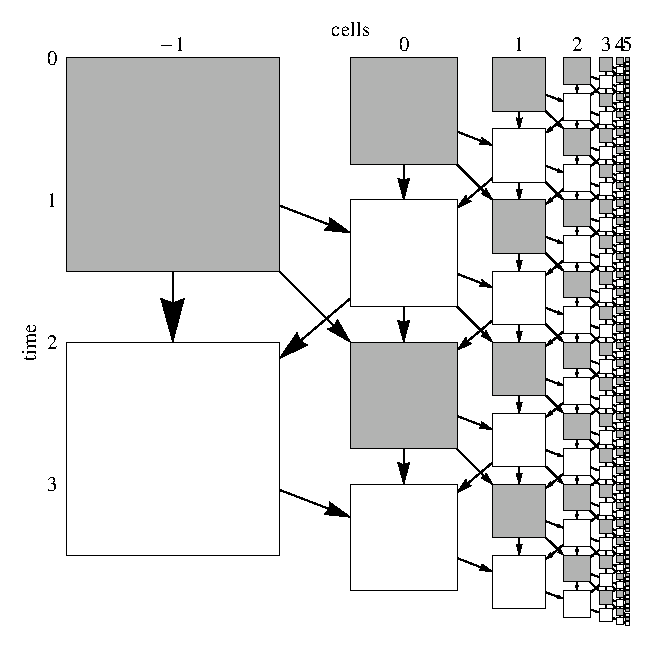
\includegraphics{2010-zsca-ssca_evolution.eps}}
\end{center}
\caption{\label{fig:ssca-evo} Evolution of a self-similar cellular automaton.
%Going to the right, cells and transition intervals are becoming progressively smaller.
%A transition of a cell that that occurs synchronously with a transition of its left neighbor is
%called coupled (gray), otherwise it is called decoupled (white).
}
\end{figure}

In what follows, we present the formal definition and the description of the update rule.

\begin{defn}
\label{def-ssca}
A self-similar cellular automaton is a tuple $A = (S, f_c, f_d)$, where $S$ is a finite set of states, and
$f_c$ and $f_d$ together represent the local rule, both functions from $S^3$ to $S$.
\end{defn}

Each cell is in a state of the state set $S$.
The state of cell $j$ is updated at times $k / 2^{j}$, where $k$ is an integer.
The cell assumes its new state at time $k / 2^{j}$ and stays in this state until $(k + 1)/2^{j}$, where
the next state change occurs.
The cycle times of a cell are the time intervals from one state transition to the next one, thus,
for cell $j$ these are the half-open intervals $[k/2^j,(k+1)/2^j)$.
This time scheduling implies that the left neighbor cell $j-1$ cycles half as fast, and the right neighbor cell $j+1$ cycles twice as fast as
the cell $j$.
At any given time, the configuration of the automaton is a mapping $c : \mathbb{Z} \rightarrow S$ that specifies the state of all cells.
We denote the state of cell $j$ at time $t$ by $c_j(t)$ and the configuration at $t$ by $c(t)$.

The state of a cell $j$ depends on the last state of the cell itself, and the last states of its left and right neighbor cell.
For notational convenience, we introduce time operators that express the temporal dependencies of a cell.
To this end, we make use of interval arithmetic.
For a scalar $\lambda \in \mathbb{R}$ and a (half-open) interval $[x,y) \subset \mathbb{R}$ set:
$\lambda + [x,y) = [\lambda + x, \lambda + y)$ and $\lambda [x,y) = [\lambda x, \lambda y)$.
We denote the unit interval $[0,1)$ by $\mathbbm{1}$.

If $T=(k + \mathbbm{1})/2^j$ specifies a cycle of cell $j$,
$T_\swarrow= (\lfloor \frac{k-1}{2} \rfloor + \mathbbm{1})/2^{j-1}$ denotes the last cycle of cell $j-1$,
$T_\downarrow= (k - 1 + \mathbbm{1})/2^j$ the last cycle of cell $j$, and
$T_\searrow =  (2k-1 + \mathbbm{1})/2^{j+1}$ the last cycle of cell $j+1$, respectively, that started before $k/2^j$.
The operator $\downarrow$ is a bijection of the set $\{(k + \mathbbm{1})/2^j| k \in \mathbb{Z} \}$, and we denote by $\uparrow$ its inverse.

The transition of cell $j$ occurs every second time at the times $2k / 2^{j} = k / 2^{j-1}$ synchronously with its left neighbor transition.
A transition of this kind is called $\emph{coupled}$, otherwise it is called $\emph{decoupled}$.
The predicate $\mathit{coupled}((k + \mathbbm{1})/2^j)$ is true if and only if the transition of the $j$-th cell at time $k / 2^{j}$ is coupled, thus,
if and only if $k$ is even.
Cells that have a state resulting from a coupled transition are filled gray in Figure \ref{fig:ssca-evo},
the cells that have a state resulting from a decoupled transition are filled white.

The self-similar cellular automaton evolves according to the following update rule.
If $T=(k + \mathbbm{1})/ 2^{j}$ is a cycle of cell $j$, the state  $c_j$ in this interval, formally described by the state function $c_j(T)$, is given by
\begin{equation}
c_j(T) = \left\{
\begin{array}{l}
f_{c}(
	c_{j - 1}(T_\swarrow),
	c_j(T_\downarrow),
	c_{j + 1}(T_\searrow)
)  \mbox{  if $\mathit{coupled}(T)$;} \\
f_{d}(
	c_{j - 1}(T_\swarrow),
	c_j(T_\downarrow),
	c_{j + 1}(T_\searrow)
) \mbox{  if $\neg\mathit{coupled}(T)$.} \\
\end{array}
\right.
\end{equation}
For any time point $t$ and any integer $j$ there exists a unique interval $T=(k + \mathbbm{1})/ 2^{j}$ such that $t \in T$.
This allows us to set $c_j(t) = c_j(T)$.

We remark that only one local rule function is necessary instead of two rule functions $f_c$ and $f_d$,
if an additional flag is added to each state that is toggled for each transition.
For the applications considered later on, the update rule given above is more compact and concise.

\subsection{Indeterminism}

The evolution of a self-similar cellular automaton might become indeterministic.
In what follows we present an example.
Consider the self-similar cellular automaton $A = (\{0,1\}, f_c, f_d)$, where $f_c$ and $f_d$ represent the left shift:
$f_c(?,?,0) = f_d(?,?,0) = 0$ and $f_c(?,?,1) = f_d(?,?,1) = 1$, where the question mark
denotes an arbitrary state.
Suppose $A$ starts at time $0$, and consider the state of cell $0$
at time $1$.
$c_0(1)$ depends on the state $c_1(1/2)$, which itself depends on $c_2(1/4)$, and so on, leading to an infinite regress.
Both possibilities $c_0(1) = c_1(1/2) = c_2(1/4) = \ldots = 0$ and $c_0(1) = c_1(1/2) = c_2(1/4) = \ldots = 1$
are consistent with the local rule and any initial configuration $c(0)$, proving that
the evolution of $A$ is indeterministic and independent of its initial configuration.

Classifying the evolution as indeterministic raises subtle questions that relate to  Thomson's lamp paradox~\cite{thom:54}.
Consider a lamp were we are instructed to switch it on for one second, to switch it off for a half second,
switch it on for a quarter second, and so on.
Naturally, one may ask whether the lamp is on or off after two seconds.
Thomson argues as follows.
If we assume that the lamp is on, it is so, because it was switched on during the sequence of jabs.
But since the sequence is infinite, there is always a switch-off operation later on in time, refuting this assumption.
The same argument holds if the lamp is off after the two seconds, leading to a contradiction,
since the lamp must be either on or off.

Thomson used this paradox to challenge the logical possibility of supertasks, but as Benacerraf \cite{benna:62} pointed out,
the paradox disappears if one accepts that the sequence of switch-on and -offs only determine the
state of the lamp in the first two seconds and only for the first two seconds.
Then both possibilities, the lamp is on or the lamp is off, are consistent with the instructions given, and the
state of the lamp after two seconds becomes indeterministic.

By formalizing the paradox, we are able to relate it more closely to self-similar cellular automata.
Let $s(t) \in \{0,1\}$ denote the state of the lamp at time $t$ and set $\neg 0 = 1$, as well as $\neg 1 =0$.
Then the set of instructions as given above can be expressed as $s(\mathbbm{1}) = 1$ and
$s(2- 1/2^{k} + \mathbbm{1}/2^{k+1}) = \neg s(2- 1/2^{k-1} + \mathbbm{1}/2^{k})$ for $k=0,1,2,\ldots$.
By altering the instructions to $s((1 + \mathbbm{1})/2^k)=\neg s((1 + \mathbbm{1})/2^{k+1})$ we obtain a time-reversed variant of the paradox,
where the zeno squeezing of the switch operations occurs now at the begin and not at the end of the considered time interval.
The state at $t=2$ cannot deduced from the set of instructions and both states $0$ and $1$ at this time are logically consistent.
Even setting $s((1 + \mathbbm{1})/2^k)=s((1 + \mathbbm{1})/2^{k+1})$ brings no rescue, since the instructions
do not allow to deduce the state for any $t > 0$ from the state at $t=0$.

In this form the paradox is similar to a form of Zeno's original paradox where the runner cannot even get started \cite{salmon-01}.
To reach the end of the racecourse the runner must first reach the midpoint of the racecourse, but before that he must first complete
the first quarter, and so on.
In order to cover any distance no matter how short, the runner must already have completed an infinite number of runs.

That the evolution is not necessarily always indeterministic can be seen be the following simple example.
Assume that the state set $S$ contains a state $q$ satisfying $f_c(?,q,?) = f_d(?,q,?) = q$.
If cell $j$ is in state $q$, it will for all times stay in this state.
Furthermore, the state of any cell to the left of cell $j$ is deterministic, since the
causal chain arising in calculating the state of any of these cells stops at cell $j$ and no infinite regress can occur.
The evolution of cells right to cell $j$ might still be indeterministic, but if the
configuration contains infinitely many cells in state $q$ the evolution is certainly deterministic.
For a more subtle example see subsection \ref{sec:block-trans}.

The following lemma reveals limitations of any deterministic evolution.
\begin{lemma}
\label{prop:det}
The state $c_i(t_2)$ of a cell $i$ of a self-similar cellular automata at time $t_2$
that was started at $t_1 < t_2$ with configuration $c(t_1)$ is deterministic if and only if
there exists an index $j$ such that $c_i(t_2)$ depends only on states $c_l(t_1)$ with $l < j$.
\end{lemma}
\begin{proof}
We choose $t_1 = 0$, $t_2 = k$, where $k$ is a positive integer, and investigate
whether the state of cell $0$ in the time interval $T=[k,k+1)$ is uniquely determined
by the deterministic states at time 0, that is the configuration $c(0)$.
The general case follows the same proof pattern.
We express a cycle of cell $i$ at time interval $T$ as pair $(i, T)$.
The set of all possible cycles starting not earlier than time $0$ is then
the set $C = \{i,(k + \mathbbm{1})/ 2^{i}| i,k \in \mathbb{Z} \mbox{ and } k \geq 0\}$.

We define a relation $\prec$ on $C$ by setting $(i_1, T_1) \prec (i_2, T_2)$ if and only if
$i_1 = i_2 - 1$ and $T_1 = {T_2}_\swarrow$, or $i_1 = i_2$ and $T_1 = {T_2}_\downarrow$, or $i_1 = i_2 + 1$ and $T_1 = {T_2}_\searrow$.
We denote the transitive closure of $\prec$ by  $\prec^*$.
This relation expresses the possible causal relationship between two transitions.

The set $P = \{(i,T^\prime) \in C| (i,T^\prime) \prec^* (0,T) \}$, the ``past light cone'' of $(0,T)$, contains $(0,T)$ as well as all cycles that
might have an effect on the state of cell $0$ in time interval $T$.
We form increasing subsets of $P$ by setting $P_j = \{(i,T^\prime) \in P| i < j\}$ for $j \geq 0$.

We call a function $s: P_j \rightarrow S$ a realization of $P_j$ if $s$ is consistent with the update rule of the self-similar
cellular automaton and $s$ matches the initial configuration at time $0$.

If we find a $P_j$ such that all realizations of it lead to the same state of cell $0$ at time interval $T$,
we know that the state is deterministic and depends only on cells of the initial configuration with index less than $j$.
Otherwise, if there is no such $P_j$, there are always two realizations $s_1$ and $s_2$ that lead to different states and which can be extended
arbitrarily to the right, resulting in two different evolutions of the self-similar cellular automata and to two different
states of cell $0$ at time interval $T$.
\end{proof}

For the sake of illustration of the implications of this lemma, consider the following example.
Let $C$ be the set of configurations, either of the form $\ldots00100\ldots$, in which exactly one $1$ with a positive index appears,
or the configuration $0^\infty$ consisting solely of $0$'s.
Assume that a self-similar automaton is started at time $0$ with a configuration $c$ in $C$.
Choose a time $t > 0$ and let $p$ be the state of cell $0$ at time $t$.
Applying the lemma, we see that there exists no local rule and hence no scale-invariant cellular automaton such
that $p$ is either $1$ if and only if $c$ is of the form $\ldots00100\ldots$, or $0$ if and only if $c=0^\infty$.
If $p$ is the result of a deterministic evolution there is an index $j$ such that
$p$ depends only on states of cells at time $0$ with index less than $j$.
This implies that the configurations $0^\infty$ and $\ldots00100\ldots$, where the index of 1 is equal to or greater than $j$,
lead to the same state $p$.

\subsection{Self-similar Cellular Automata with Quiescent State}
\label{sec:quies}

The indeterminism of self-similar cellular automata can be restricted by considering the following subclass
which adds a quiescent state to the original concept and allows for lattices
that contain only a finite number of cells.

\begin{defn}
A self-similar cellular automaton with quiescent state is a tuple $A = (S, f_c, f_d, q)$, where
$S$, $f_c$, and $f_d$ are defined as in Def.~\ref{def-ssca}, and
$q$ in $S$ is a distinguished state, the quiescent state,
satisfying $f_c(q,q,q) = f_d(q,q,q) = q$.
\end{defn}

If the automaton has a quiescent state, we allow for finite or half-infinite lattices that start with cell $0$.
The update rule of the automaton is adapted to cope with cells that have no left or right neighbor.
Furthermore we allow the lattice to grow to the right.
If either the left or right neighbor is missing, the state of the missing neighbor is assumed to be the quiescent state.
In case of a finite lattice, consisting of $n+1$ cells $0, 1, \ldots, n$, we allow the lattice to grow,
if the state of cell $n$ differs from the quiescent state.
If cell $n$ at time $k / 2^n$ changes to a state, different from the quiescent state, a new cell $n+1$ is added to
the lattice.
This new cell $n+1$ is initialized with the quiescent state and attached to cell $n$.
The first update of this new cell occurs at time $k / 2^n + 1/2$.

We remark that the evolution of a finite lattice is always deterministic as long as the lattice stays finite, since no infinite regress can occur.
However, a finite lattice can grow to infinity and the evolution can become indeterministic as described in the preceding subsection.


\subsection{Block Transformations}
\label{sec:block-trans}

If the state set becomes larger, the specification of the values for the local rules $f_c$ and $f_d$ for all possible arguments
is rather lengthy.
Some self-similar cellular automata allow an alternative specification.
A coupled transition of two neighbor cells can perform a simultaneous state change of the two cells.
If the state changes of these two neighbor cells are independent of their other neighbors,
we can specify the state changes as a transformation of one state pair into another.
Let $z_1, z_2, z_1^\prime, z_2^\prime$ be elements in $S$.
We call a mapping of the form $z_1 \: z_2 \mapsto z_1^\prime \: z_2^\prime$ a block transformation.
The block transformation $z_1 \: z_2 \mapsto z_1^\prime \: z_2^\prime$ defines
 a function mapping of the form
$
f_c(x, z_1, z_2) = f_d(x, z_1, z_2) = z_1^\prime
$
and
$
f_c(z_1, z_2,y) = z_2^\prime
$
for all $x, y$ in $S$.
Furthermore, we will also allow block transformations that might be ambiguous for certain configurations.
Consider the block transformations
$z_1 \: z_2 \mapsto z_1^\prime \: z_2^\prime$
and
$z_2 \: z_3 \mapsto z_2^{\prime\prime} \: z_3^\prime$
that might lead to an ambiguity for a configuration that contains $z_1z_2z_3$.
Instead of resolving these ambiguities in a formal way, we will restrict our attention to
configurations that are unambiguous.

Consider the self-similar cellular automaton $A = (S, f_c, f_d)$, where $S$ is the set
$ (\{0,1\} \times \{<,>\}) \cup \{\filledmedsquare\}$.
If $q \in \{0,1\}$, we write $q_<$ for $(q,<)$, and $q_>$ for $(q,>)$, respectively.
We specify  $f_c$ and $f_d$ by the following block transformations
\begin{equation}
0_>\filledmedsquare \mapsto 0_<\filledmedsquare, \: 1_>\filledmedsquare \mapsto 1_<\filledmedsquare, \: \filledmedsquare0_< \mapsto \filledmedsquare0_>, \: \filledmedsquare1_< \mapsto \filledmedsquare1_>;
\end{equation}
\begin{equation}
0_> 0_< \mapsto 0_< 0_>, \:  1_> 0_< \mapsto 0_< 1_>, \: 0_> 1_< \mapsto 1_< 0_>, \mbox{ and } 1_> 1_< \mapsto 1_< 1_>;
\end{equation}
together with the convention, that a cell remains in its previous state, if no block transformation is applicable.
Let $A$ be started with a configuration of the form
$\ldots \filledmedsquare \filledmedsquare {q_1}_> {q_2}_< {q_3}_> {q_4}_< \ldots {q_{n-1}}_> {q_{n}}_<  \filledmedsquare \filledmedsquare \ldots$, where all $q_i$ are in  $\{0,1\}$.
It is easy to see that the evolution of $A$ is deterministic and that
$A$ runs the one-dimensional billard ball model of Margolus \cite{margolus-billard}.
Furthermore, the construction shows that a self-similar cellular automaton can simulate any 3-site
one-dimensional cellular automaton.


\section{Construction of a Hypercomputer}
\label{sec:hypercomputer}

\subsection{Preliminaries}
\label{sec:hc-spec}

In what follows we will construct a hypercomputers based on a self-similar cellular automaton.
This hypercomputer simulates a Turing machine and is capable of performing infinitely many steps
of the Turing machine in finite time.
We assume the following Turing machine model as described in \cite{hopcroft}.

Formally, a {\em Turing machine}  is a tuple
$M = (Q, \Sigma, \Gamma, \delta, q_0, B, F)$,
where $Q$ is the finite set of states, $\Gamma$ is the finite set of tape symbols,
$\Sigma \subset \Gamma$ is the set of input symbols, $q_0 \in Q$ is the start state,
$B \in \Gamma \backslash \Sigma$ is the blank, and $F \subset Q$ is the set of final states.
The next move function or transition function $\delta$ is a mapping from
$Q \times \Gamma$ to $Q \times \Gamma \times \{L, R\}$, which may be undefined for some arguments.

The Turing machine $M$ works on a tape divided into cells that has a leftmost cell but is infinite to the right.
Let $\delta(q, a) = (p, b, D)$.
One step (or move) of $M$ in state $q$ and the head of $M$ positioned over input symbol $a$
consists of the following actions:
scanning input symbol $a$, replacing symbol $a$ by $b$,
entering state $p$ and moving the head one cell either to the left ($D=L$) or to the right ($D=R$).
In the beginning, $M$ starts in state $q_0$ with a tape that is initialized with an input word $w \in \Sigma^*$,
starting at the leftmost cell, all other cells blank,
and the head of $M$ positioned over the leftmost cell.

\begin{figure}
\begin{center}
\renewcommand{\arraystretch}{1}
\begin{tabular}{c|ccccc}
& \multicolumn{5}{c}{ Symbol} \\
State & 0 & 1 & $X$ & $Y$ & $B$ \\ \hline
$p$ & $(q,X,R)$ & ---         & ---         & $(s,Y,R)$ & ---         \\
$q$ & $(q,0,R)$ & $(r,Y,L)$ & ---         & $(q,Y,R)$ & ---         \\
$r$ & $(r,0,L)$ & ---         & $(p,X,R)$ & $(r,Y,L)$ & ---         \\
$s$ & ---         & ---         & ---         & $(s,Y,R)$ & $(t,B,R)$ \\
$t$ & ---         & ---         & ---         & ---         & ---         \\
\end{tabular}
\end{center}
\caption{\label{fig:example-delta}The function $\delta$.}
\end{figure}

After presenting the construction of a hypercomputer, we will use the following simple example
to illustrate its working.
Let $L$ be the formal language consisting of strings with $n$ 0's, followed by $n$ 1's:
$L = \{0^n1^n | n \geq 1\}$.
A Turing machine that accepts this language is given by
$M = (\{p, q, r, s, t\}, \{0,1\}, \{0,1,X,Y,B\}, \delta, p, B, \{t\})$, see \cite{hopcroft},
with the transition function depicted in Figure \ref{fig:example-delta}.
Note that $L$ is a context-free language, but $M$ will serve for demonstration purposes.
The computation of $M$ on input $01$ is given below:
\[
p01 \vdash Xq1  \vdash  rXY  \vdash  XpY  \vdash  XYs  \vdash XYt.
\]

\subsection{The Stop and Go Hypercomputer Construction}
\label{sec:stop-and-go}

Given an arbitrary Turing machine $M$ we construct a self-similar cellular automaton with quiescent state $A_M = (S, f_c, f_d, \Box)$
that simulates $M$.

Set $T=(Q \times \{\smalltriangleleft, \smalltriangleright\}) \cup \Gamma$.
Then the state set $S$ of $A_M$ is given by
\[
S = T \cup (T \times \{\blacktriangleright\}) \cup \{\Box, \filledmedsquare, \diamond \}.
\]
For an element $q$ in $Q$, we write $q^\smalltriangleleft$ for $(q,\smalltriangleleft)$ and $q^\smalltriangleright$ for $(q,\smalltriangleright)$, respectively.
We write $x_\blacktriangleright$ for an element $(x, \blacktriangleright)$ in $T \times \{\blacktriangleright\}$.
The local rule of $A_M$ is specified by the following block transformations, where $x$ denotes an element in $T$, $a$ and $b$ are in
$\Gamma$ and $q$ and $p$ are in $Q$.
If no block transformation is applicable, a cell remains in its previous state.
\begin{enumerate}
\item Set
\begin{equation}
\label{eq:del_x}
\filledmedsquare \: x \mapsto\filledmedsquare \: x_\blacktriangleright \mbox{ if } x \not = q^\smalltriangleleft;
\end{equation}
\begin{equation}
\label{eq:x_-}
x_\blacktriangleright \: \diamond \mapsto \diamond\: x;
\end{equation}
\begin{equation}
\label{eq:a_b}
a \: b \mapsto a \: b_\blacktriangleright;
\end{equation}
\begin{equation}
q^\smalltriangleleft \: a \mapsto q^\smalltriangleleft \: a_\blacktriangleright;
\end{equation}
\begin{equation}
a \: q^\smalltriangleright \mapsto a \: q^\smalltriangleright_\blacktriangleright;
\end{equation}
\begin{equation}
\label{eq:a_quies}
x \: \Box \mapsto x \: \diamond \mbox{ if } x \not = q^\smalltriangleright;
\end{equation}
\begin{equation}
\label{eq:B1}
q^\smalltriangleright \: \Box \mapsto q^\smalltriangleright \: B_\blacktriangleright;
\end{equation}
\begin{equation}
\label{eq:B2}
B_\blacktriangleright \: \Box \mapsto \diamond \: B;
\end{equation}
\begin{equation}
\label{eq:del_-}
\filledmedsquare \: \diamond \mapsto \diamond \: \filledmedsquare.
\end{equation}
\item If $\delta(q,a) = (p,b,R)$ set
\begin{equation}
\label{eq:head1}
q^\smalltriangleright \: a \mapsto b \: p^\smalltriangleright_\blacktriangleright;
\end{equation}
\begin{equation}
\label{eq:head2}
a \: q^\smalltriangleleft \mapsto b \: p^\smalltriangleright_\blacktriangleright.
\end{equation}
\item If $\delta(q,a) = (p,b,L)$ set
\begin{equation}
\label{eq:head3}
q^\smalltriangleright \: a \mapsto p^\smalltriangleleft \: b_\blacktriangleright;
\end{equation}
\begin{equation}
\label{eq:head4}
a \: q^\smalltriangleleft \mapsto p^\smalltriangleleft \: b_\blacktriangleright.
\end{equation}
\end{enumerate}

\begin{figure}
\begin{center}
\small     {
\renewcommand{\arraystretch}{0.9}
\begin{tabular}{r|p{4mm}@{}p{4mm}@{}p{4mm}@{}p{4mm}@{}p{4mm}@{}p{4mm}@{}p{4mm}@{}p{4mm}@{}p{4mm}@{}p{4mm}@{}p{4mm}@{}p{4mm}@{}p{4mm}@{}p{4mm}@{}p{4mm}@{}p{4mm} }
& \multicolumn{15}{c}{cells} \\
\multicolumn{1}{c|}{time}    &0 &1 & 2 & 3 & 4 & 5 & 6 & 7 & 8 & 9 &10 &11 &12 &13 &14\\ \hline
$0.000000000000_2$ & $\filledmedsquare$ & $p^\smalltriangleright$ & $\diamond$ & $0$ & $\diamond$ & $1$ & $\diamond$ &  &  &  &  &  & \\
$1.000000000000_2$ & $\filledmedsquare$ & $p^\smalltriangleright_\blacktriangleright$ & $\diamond$ & $0$ & $\diamond$ & $1$ & $\diamond$ & $\Box$ &  &  &  &  & \\
$1.100000000000_2$ & $\filledmedsquare$ & $\diamond$ & $p^\smalltriangleright$ & $0$ & $\diamond$ & $1$ & $\diamond$ & $\Box$ &  &  &  &  & \\
$1.110000000000_2$ & $\filledmedsquare$ & $\diamond$ & $X$ & $q^\smalltriangleright_\blacktriangleright$ & $\diamond$ & $1$ & $\diamond$ & $\Box$ &  &  &  &  & \\
$1.111000000000_2$ & $\filledmedsquare$ & $\diamond$ & $X$ & $\diamond$ & $q^\smalltriangleright$ & $1$ & $\diamond$ & $\Box$ &  &  &  &  & \\
$1.111100000000_2$ & $\filledmedsquare$ & $\diamond$ & $X$ & $\diamond$ & $r^\smalltriangleleft$ & $Y_\blacktriangleright$ & $\diamond$ & $\Box$ &  &  &  &  & \\
$1.111110000000_2$ & $\filledmedsquare$ & $\diamond$ & $X$ & $\diamond$ & $r^\smalltriangleleft$ & $\diamond$ & $Y$ & $\Box$ &  &  &  &  & \\
$1.111111000000_2$ & $\filledmedsquare$ & $\diamond$ & $X$ & $\diamond$ & $r^\smalltriangleleft$ & $\diamond$ & $Y$ & $\diamond$ & $\Box$ &  &  &  & \\
$10.000000000000_2$ & $\diamond$ & $\filledmedsquare$ & $X$ & $\diamond$ & $r^\smalltriangleleft$ & $\diamond$ & $Y$ & $\diamond$ & $\Box$ &  &  &  & \\
$10.100000000000_2$ & $\diamond$ & $\filledmedsquare$ & $X_\blacktriangleright$ & $\diamond$ & $r^\smalltriangleleft$ & $\diamond$ & $Y$ & $\diamond$ & $\Box$ &  &  &  & \\
$10.110000000000_2$ & $\diamond$ & $\filledmedsquare$ & $\diamond$ & $X$ & $r^\smalltriangleleft$ & $\diamond$ & $Y$ & $\diamond$ & $\Box$ &  &  &  & \\
$10.111000000000_2$ & $\diamond$ & $\filledmedsquare$ & $\diamond$ & $X$ & $p^\smalltriangleright_\blacktriangleright$ & $\diamond$ & $Y$ & $\diamond$ & $\Box$ &  &  &  & \\
$10.111100000000_2$ & $\diamond$ & $\filledmedsquare$ & $\diamond$ & $X$ & $\diamond$ & $p^\smalltriangleright$ & $Y$ & $\diamond$ & $\Box$ &  &  &  & \\
$10.111110000000_2$ & $\diamond$ & $\filledmedsquare$ & $\diamond$ & $X$ & $\diamond$ & $Y$ & $s^\smalltriangleright_\blacktriangleright$ & $\diamond$ & $\Box$ &  &  &  & \\
$10.111111000000_2$ & $\diamond$ & $\filledmedsquare$ & $\diamond$ & $X$ & $\diamond$ & $Y$ & $\diamond$ & $s^\smalltriangleright$ & $\Box$ &  &  &  & \\
$10.111111100000_2$ & $\diamond$ & $\filledmedsquare$ & $\diamond$ & $X$ & $\diamond$ & $Y$ & $\diamond$ & $s^\smalltriangleright$ & $B_\blacktriangleright$ & $\Box$ &  &  & \\
$10.111111110000_2$ & $\diamond$ & $\filledmedsquare$ & $\diamond$ & $X$ & $\diamond$ & $Y$ & $\diamond$ & $s^\smalltriangleright$ & $\diamond$ & $B$ & $\Box$ &  & \\
$10.111111111000_2$ & $\diamond$ & $\filledmedsquare$ & $\diamond$ & $X$ & $\diamond$ & $Y$ & $\diamond$ & $s^\smalltriangleright$ & $\diamond$ & $B$ & $\diamond$ & $\Box$ & \\
$11.000000000000_2$ & $\diamond$ & $\diamond$ & $\filledmedsquare$ & $X$ & $\diamond$ & $Y$ & $\diamond$ & $s^\smalltriangleright$ & $\diamond$ & $B$ & $\diamond$ & $\Box$ & \\
$11.010000000000_2$ & $\diamond$ & $\diamond$ & $\filledmedsquare$ & $X_\blacktriangleright$ & $\diamond$ & $Y$ & $\diamond$ & $s^\smalltriangleright$ & $\diamond$ & $B$ & $\diamond$ & $\Box$ & \\
$11.011000000000_2$ & $\diamond$ & $\diamond$ & $\filledmedsquare$ & $\diamond$ & $X$ & $Y$ & $\diamond$ & $s^\smalltriangleright$ & $\diamond$ & $B$ & $\diamond$ & $\Box$ & \\
$11.011100000000_2$ & $\diamond$ & $\diamond$ & $\filledmedsquare$ & $\diamond$ & $X$ & $Y_\blacktriangleright$ & $\diamond$ & $s^\smalltriangleright$ & $\diamond$ & $B$ & $\diamond$ & $\Box$ & \\
$11.011110000000_2$ & $\diamond$ & $\diamond$ & $\filledmedsquare$ & $\diamond$ & $X$ & $\diamond$ & $Y$ & $s^\smalltriangleright$ & $\diamond$ & $B$ & $\diamond$ & $\Box$ & \\
$11.011111000000_2$ & $\diamond$ & $\diamond$ & $\filledmedsquare$ & $\diamond$ & $X$ & $\diamond$ & $Y$ & $s^\smalltriangleright_\blacktriangleright$ & $\diamond$ & $B$ & $\diamond$ & $\Box$ & \\
$11.011111100000_2$ & $\diamond$ & $\diamond$ & $\filledmedsquare$ & $\diamond$ & $X$ & $\diamond$ & $Y$ & $\diamond$ & $s^\smalltriangleright$ & $B$ & $\diamond$ & $\Box$ & \\
$11.011111110000_2$ & $\diamond$ & $\diamond$ & $\filledmedsquare$ & $\diamond$ & $X$ & $\diamond$ & $Y$ & $\diamond$ & $B$ & $t^\smalltriangleright_\blacktriangleright$ & $\diamond$ & $\Box$ & \\
$11.011111111000_2$ & $\diamond$ & $\diamond$ & $\filledmedsquare$ & $\diamond$ & $X$ & $\diamond$ & $Y$ & $\diamond$ & $B$ & $\diamond$ & $t^\smalltriangleright$ & $\Box$ & \\
$11.011111111100_2$ & $\diamond$ & $\diamond$ & $\filledmedsquare$ & $\diamond$ & $X$ & $\diamond$ & $Y$ & $\diamond$ & $B$ & $\diamond$ & $t^\smalltriangleright$ & $B_\blacktriangleright$ & $\Box$\\
$11.011111111110_2$ & $\diamond$ & $\diamond$ & $\filledmedsquare$ & $\diamond$ & $X$ & $\diamond$ & $Y$ & $\diamond$ & $B$ & $\diamond$ & $t^\smalltriangleright$ & $\diamond$ & $B$ & $\Box$\\
$11.011111111111_2$ & $\diamond$ & $\diamond$ & $\filledmedsquare$ & $\diamond$ & $X$ & $\diamond$ & $Y$ & $\diamond$ & $B$ & $\diamond$ & $t^\smalltriangleright$ & $\diamond$ & $B$ & $\diamond$ & $\Box$\\
$11.100000000000_2$ & $\diamond$ & $\diamond$ & $\diamond$ & $\filledmedsquare$ & $X$ & $\diamond$ & $Y$ & $\diamond$ & $B$ & $\diamond$ & $t^\smalltriangleright$ & $\diamond$ & $B$ & $\diamond$ & $\Box$\\
$11.101000000000_2$ & $\diamond$ & $\diamond$ & $\diamond$ & $\filledmedsquare$ & $X_\blacktriangleright$ & $\diamond$ & $Y$ & $\diamond$ & $B$ & $\diamond$ & $t^\smalltriangleright$ & $\diamond$ & $B$ & $\diamond$ & $\Box$\\
$11.101100000000_2$ & $\diamond$ & $\diamond$ & $\diamond$ & $\filledmedsquare$ & $\diamond$ & $X$ & $Y$ & $\diamond$ & $B$ & $\diamond$ & $t^\smalltriangleright$ & $\diamond$ & $B$ & $\diamond$ & $\Box$\\
$11.101110000000_2$ & $\diamond$ & $\diamond$ & $\diamond$ & $\filledmedsquare$ & $\diamond$ & $X$ & $Y_\blacktriangleright$ & $\diamond$ & $B$ & $\diamond$ & $t^\smalltriangleright$ & $\diamond$ & $B$ & $\diamond$ & $\Box$\\
$11.101111000000_2$ & $\diamond$ & $\diamond$ & $\diamond$ & $\filledmedsquare$ & $\diamond$ & $X$ & $\diamond$ & $Y$ & $B$ & $\diamond$ & $t^\smalltriangleright$ & $\diamond$ & $B$ & $\diamond$ & $\Box$\\
$11.101111100000_2$ & $\diamond$ & $\diamond$ & $\diamond$ & $\filledmedsquare$ & $\diamond$ & $X$ & $\diamond$ & $Y$ & $B_\blacktriangleright$ & $\diamond$ & $t^\smalltriangleright$ & $\diamond$ & $B$ & $\diamond$ & $\Box$\\
$11.101111110000_2$ & $\diamond$ & $\diamond$ & $\diamond$ & $\filledmedsquare$ & $\diamond$ & $X$ & $\diamond$ & $Y$ & $\diamond$ & $B$ & $t^\smalltriangleright$ & $\diamond$ & $B$ & $\diamond$ & $\Box$\\
$11.101111111000_2$ & $\diamond$ & $\diamond$ & $\diamond$ & $\filledmedsquare$ & $\diamond$ & $X$ & $\diamond$ & $Y$ & $\diamond$ & $B$ & $t^\smalltriangleright_\blacktriangleright$ & $\diamond$ & $B$ & $\diamond$ & $\Box$\\
$11.101111111100_2$ & $\diamond$ & $\diamond$ & $\diamond$ & $\filledmedsquare$ & $\diamond$ & $X$ & $\diamond$ & $Y$ & $\diamond$ & $B$ & $\diamond$ & $t^\smalltriangleright$ & $B$ & $\diamond$ & $\Box$\\
\end{tabular}
}
\end{center}
\caption{\label{fig:example-stopandgo}A computation of $A_M$ on input $01$.}
\end{figure}


To simulate $M$ on the input $a_1 \ldots a_n$, $A_M$ is started with the configuration
$\filledmedsquare q_0^\smalltriangleright \diamond a_1 \diamond a_2 \diamond \ldots \diamond a_n \diamond$.
Note that according to Subsection \ref{sec:quies} $A_M$ starts with a finite configuration and that
whenever the rightmost cell of the configuration differs from the quiescent state a new cell is appended to the
lattice.
Figure \ref{fig:example-stopandgo} depicts the computation of $A_M$ on the Turing machine input $01$ showing
the configurations where a state change occurred except the ones where only a cell with quiescent state was appended to
the lattice.

The construction of $A_M$ achieves two goals.
On the one hand, it simulates correctly the Turing machine $M$, on the other hand
the simulation of the Turing machine is interleaved with a shift of the tape content and the head
of the Turing machine to the right, faster-cycling cells, thereby achieving a progressive acceleration
of the simulation.

We give an informal description of the construction.
A symbol in $Q \times \{\smalltriangleleft, \smalltriangleright\}$ acts as head of the Turing machine, either
facing to the left ($\smalltriangleleft$) or the right ($\smalltriangleright$), thereby indicating
whether either the tape symbol to the left or to the right is scanned next.
The shift to the right has to be performed in a controlled way to avoid that tape symbols to the right
are moving faster than symbols to the left, thereby spreading the tape content.

A controlled shift is achieved by a stop-and-go synchronization in form of the two states $x$ and $x_\blacktriangleright$
of each tape symbol and the head.
The shift starts at the left delimiter $\filledmedsquare$. If
adjacent to a symbol $x$ block transformation \ref{eq:del_x} changes the state of $x$ to
$x_\blacktriangleright$.
A symbol $x_\blacktriangleright$ moves one cell to the right, thereby changing its state back to $x$ and
swapping place with $\diamond$.
If two symbols $x$ and $y$ in $T$ are adjacent the right symbol is excited to state $y_\blacktriangleright$.
If one of them is a tape symbol and the other one is a head facing the tape symbol, one step of the Turing machine is simulated
according to block transformations \ref{eq:head1} -- \ref{eq:head4}.
A shift-over ends when the left delimiter $\filledmedsquare$ swaps place with the spacer $\diamond$ due to
block transformation \ref{eq:del_-}.

\subsection{Results}

The following proposition is analogous to Theorem 2 of \cite{2008-sica}, where
a formal and lengthy proof was given.
Here we outline the proof by giving exemplary derivations without performing all case distinctions in detail.
\begin{prop}If the Turing machine $M$ halts on input $w$, $A_M$ halts in less than $4$ time units.
If $M$ does not halt, $A_M$ enters at time $4$ the configuration $\diamond^\infty$.
\end{prop}
\begin{proof}
To prove the proposition about the timing, we first consider the evolution of the self-similar cellular automaton
$B = (\{\ a, a_\blacktriangleright, \Box, \filledmedsquare, -\},  f_c, f_d, \Box)$ with initial
configuration $\filledmedsquare a \diamond a \diamond \cdots\diamond  a \diamond$, where $a$ is an arbitrary input symbol from $\Sigma$.
Only block transformations \ref{eq:del_x}, \ref{eq:x_-}, \ref{eq:a_b},
\ref{eq:a_quies}, and \ref{eq:del_-} are required to describe the evolution of $B$.
We claim that a configuration $\diamond^m \filledmedsquare a \diamond a \diamond \cdots\diamond  a \diamond$,
where $m$ is a positive integer,
evolves in $2^{1-m}$ cycles of cell 0 to the configuration $\diamond^{m+1} \filledmedsquare a \diamond a \diamond \cdots\diamond  a \diamond$.
We perform the calculation for $m=0$, the initial configuration, the general case follows from the scale-invariance and
the fact that leading $\diamond$'s have no impact on the evolution. We use the notation $c_1 \stackrel{t}{\longrightarrow}  c_2$
to denote that configuration $c_1$ changed at time $t$ to configuration $c_2$.

We obtain
$\filledmedsquare a \diamond a \diamond \cdots
\stackrel{1}{\longrightarrow} \filledmedsquare a_\blacktriangleright \diamond a \diamond \cdots
\stackrel{1.1}{\longrightarrow} \filledmedsquare \diamond a a \diamond\cdots
\stackrel{1.11}{\longrightarrow} \filledmedsquare \diamond a a_\blacktriangleright \diamond\cdots
\stackrel{1.111}{\longrightarrow} \filledmedsquare \diamond a \diamond a\cdots
$.
The final steps before the whole configuration has shifted one cell to the right are
$
\filledmedsquare \ldots a a \diamond \Box
\stackrel{1.1 \ldots 1}{\longrightarrow} \filledmedsquare \diamond  \ldots a a_\blacktriangleright \diamond \Box
\stackrel{1.1 \ldots 11}{\longrightarrow} \filledmedsquare \diamond \ldots a \diamond a \Box
\stackrel{1.1 \ldots 111}{\longrightarrow} \filledmedsquare \diamond \ldots a \diamond a \diamond
\stackrel{1.1 \ldots 1111}{\longrightarrow} \filledmedsquare \diamond \ldots a \diamond a \diamond \Box
\stackrel{2}{\longrightarrow} \diamond \filledmedsquare \ldots a \diamond a \diamond \Box
$.

A similar but more lengthy calculation, not done here, can be performed for $A_M$ showing
that in the regular case a configuration $\diamond^m \filledmedsquare a_1 \diamond a_2 \diamond \cdots \diamond a_i \diamond q^d \diamond a_{i+1} \diamond \cdots a_n \diamond$
evolves in $2^{1-m}$ time units to a configuration
$\diamond^{m+1} \filledmedsquare b_1 \diamond b_2 \diamond \cdots \diamond b_j \diamond p^{e} \diamond b_{j+1} \diamond \cdots b_n \diamond$,
where $d$ and $e$ are in $\{\smalltriangleleft, \smalltriangleright\}$.
The following exceptions have to be considered.
If $M$ halts, none of the rules \ref{eq:head1} -- \ref{eq:head4} can be applied and $A_M$ enters a final configuration
as soon as the shift reaches the head.
The other exception occurs when the head $q$ tries to scan a symbol right from the end of the simulated tape, i.e., when a
configuration of the form $\cdots q^\smalltriangleright \Box$ occurs.
In this case the symbol $B$, the blank,  has to be appended to the end of the simulated tape.
This tape extension is the net effect of the block transformations \ref{eq:B1} and \ref{eq:B2}, see the space-time diagram of
the example in Figure \ref{fig:example-stopandgo} at time $10.111111_2$.
Note that extending the simulated tape by a blank does not alter the time behavior of the overall shift.
Hence, if $M$ does not halt, $A_M$ reaches after $2 + 2/2 + 2/4 + \ldots = 4$ time units the final configuration $\diamond^\infty$.

The proof of the correctness of the simulation starts by  mapping configurations of $A_M$ to
instantaneous descriptions of $M$.
For instance, the configuration
$\diamond^m \filledmedsquare a_1 \diamond a_2 \diamond \cdots \diamond a_i \diamond q^d \diamond a_{i+1} \diamond \cdots a_n \diamond$
maps to the instantaneous description $a_1a_2 \cdots a_i q a_{i+1} \cdots a_n$, if $d=\smalltriangleright$
and to  $a_1a_2 \cdots q a_i a_{i+1} \cdots a_n$ if $d=\smalltriangleleft$.
By showing that each block transformation that is applied either does not alter the instantaneous description
or leads to the	successive instantaneous description of $M$, the correctness is proven.

We end the outline of the proof by remarking that each shift of the tape content by one cell to the right simulates at least one step of the Turing machine.
\end{proof}
Since $A_M$ is capable of performing infinite many steps of $M$ in finite time the following proposition follows easily.
\begin{cor}
If $M_U$ is a universal Turing machine, then $A_{M_U}$ solves the halting problem for Turing machines.
\end{cor}

We imagine that an operator initializes the first cells of the self-similar automaton with the input of the calculation.
Ideally, in case that the simulated Turing machine has halted, the self-similar automaton should propagate this fact
back to the left cells.
But by Lemma \ref{prop:det} we know that there is no deterministic way to do this.
Therefore the operator would have to scan a possible infinite numbers of cells to decide whether the Turing machine has
halted or not.
The following section presents a closely related model of computation that avoids the indeterminism in the infinite case.


\section{Self-similar Petri Nets}
\label{sec:petri}

\begin{figure*}
\begin{center}
\includegraphics[scale=0.6]{2010-zsca-ssca_petri.eps}
\end{center}
\caption{\label{fig:petri} Underlying graph of a self-similar Petri net \cite{2008-sica}.}
\end{figure*}

Self-similar Petri nets result from carrying over the self-similar cellular automaton model to the theory of Petri nets.
We refer to \cite{Murata89} for a concise introduction to Petri net theory, here we give only a very short
summary to settle the terminology.

The underlying graph of a Petri net is a directed, weighted, bipartite graph consisting of two kind of nodes,
called transitions and places.
Figure \ref{fig:petri} depicts the underlying graph of a self-similar Petri net, drawing
transitions as boxes and places as circles.
A place that has an arc to a transition is an input place of this transition,
if the arc is from the transition to the place, the place is an output place.
Arcs are labeled with their weights.

Places hold so-called tokens.
A marking assigns to each place a number, the number of tokens in this place.
The marking in a Petri net is changed according to the following transition (firing) rule:
\begin{enumerate}
\item A transition $t$ is enabled if each input place $p$ of $t$ is marked with at
least $w(p,t)$ tokens, where $w(p,t)$ is the weight of the arc from $p$ to $t$.
\item An enabled transition $t$ may fire. A firing removes $w(p,t)$ tokens from each input place $p$,
and adds $w(t,p)$ tokens to each output place $p$ of $t$, where $w(t,p)$ is the weight
of the arc from $t$ to $p$.
\end{enumerate}

Self-similar Petri nets are both colored Petri nets and marked graphs.
The first says that the tokens of the Petri net carry values and that
the firing rule is adapted such that the value of an output token is determined by the values of the input tokens.
The latter says that each place is the input place and the output place of at most one transition, which
makes the Petri net deterministic.

We will informally describe how the concepts of self-similar cellular automata are mapped to self-similar Petri nets,
for a formal treatment we refer to \cite{2008-sica}.
The states of a self-similar cellular automaton are mapped to the values of the tokens.
The transition of the self-similar Petri net uses the values of the input tokens to calculate
the value of the output tokens according to the local rules $f_c$ and $f_d$ that are carried over from self-similar cellular automata.

A firing of cell $n$ consumes two tokens of cell $n+1$ and puts two new tokens in the input place of cell $n+1$.
Since cell $n+1$ consumes per firing only one token from cell $n$, and puts only one token in the input place of cell $n$,
cell $n+1$ must fire twice before cell $n$ can fire again.
As we can see, the doubling of cycles from one cell to its right neighbor works now by a synchronisation mechanism without reference to
an external clock.

In analogy to self-similar cellular automata with quiescent state, a self-similar Petri net
is started with a finite number of cells and is allowed to grow to the right, whenever the rightmost cell
calculates a token value different from the quiescent state.

To ensure the liveness of the self-similar Petri net the left- and rightmost cells
obey the the following boundary conditions.
Each firing of the leftmost cell puts one token in its left input place, each firing of the rightmost cell
puts two tokens in its right input place.

If the self-similar Petri net is started with a certain marking and proper token values it can be shown
that self-similar Petri nets and self-similar cellular automata feature a step-by-step equivalence for calculations that
involve only a finite number of steps.

Self-similar Petri nets work without any reference to an external clock, but it is possible to impose a time scheduling
leading to timed self-similar Petri nets.
If we require that transition $n$ always fires when it is enabled and that the firing process, which includes
the consumption and production of tokens, takes no longer than $1/2^n$ time units, we obtain
the same time model as for self-similar cellular automata.

The construction of Subsection \ref{sec:stop-and-go} can also be applied to timed self-similar Petri nets,
leading to a self-similar Petri net $N_M$ that simulates a Turing machine $M$.
In contrast to self-similar cellular automata, the evolution of a Petri net can stop.
This happens when no transition is enabled.
In \cite{2008-sica} it was proven that the Petri net stops when the Turing machine does not halt, thereby avoiding
the indeterminismn of self-similar cellular automata.

\section{Summary}

We have reviewed two recently introduced models of computation, both based on an infinite,
progressive tessellation of space and time.
Space and time tessellations are the same as the paradox of the runner that cannot reach the end of a racecourse,
imagined by Zeno more than 2500 years ago.

Both computing models are capable of hypercomputing, even if they differ in the limit of non-halting Turing machine simulations.
Thus we were able to replace the sequence of shrinking Turing machines that Davies \cite{Davies01} used to construct a hypercomputer
within a Newtonian universe,
by a sequence of shrinking finite automata (or Petri net transitions).

If properly programmed, self-similar cellular automata enter a final quiescent configuration and loop  forever there; if not,
they end up in indeterminism.

The underlying graph of a self-similar Petri net grows to
infinity, if the simulated Turing machine does not halt.
Since there is no longer a rightmost cell that obeys the boundary condition that guaranteed the liveness
of the system for the finite case, the self-similar Petri net stops.
Thus, self-similar Petri nets halt if and only if the simulated Turing machine does not halt.

The main contributions of this paper are a proposition about the indeterminism of self-similar cellular automata
and a simplified construction of a hypercomputer.
The stop-and-go construction requires only one synchronization pulse that travels from the left delimiter to the right end
of the configuration, instead of the zigzagging pulse in \cite{2008-sica}.
It takes now only 4 time units instead of 6 to perform infinitely many steps of the simulated Turing machine.
Furthermore, the construction is conceptually simpler and the number of states of the self-similar cellular automaton
was reduced.
A drawback of the stop-and-go construction is the fact that the initial configuration consumes now roughly twice the
number of cells than the zigzag construction.

The construction of simple hypercomputers based on self-similar cellular automata that simulate a universal
Turing machine is an interesting research problem, see \cite{turlough-09} for simple universal Turing machines.
We used self-similar cellular automata mainly as a vehicle to construct a hypercomputer, but an analytical and/or phenomenological
investigation of this new model of computation should allow to gain further insights and strengthen the connection to
cellular automata.
It might also be possible to generalize those two models of computation using graph grammars, graph transformation or
graph rewriting systems, see e.g., \cite{ehrig-06}.

Both models suffer from what we call the {\em response problem}.
We imagine an operator that initializes the very first cells of either of the two machines with the input of the
calculation and then starts the machine.
Ideally, after some finite amount of time the operator would obtain an answer that is again written
to the first cells of the machine.
Thus, the response problem is the problem of propagating the final status of the simulated Turing machine,
 which is either ``halt" or ``non-halt," back to the cells with lower index,
say cell $0$.

Both models fail to solve the response problem; yet due to different reasons.
If we extend the rules of the self-similar cellular automaton to propagate a response back to the left cells,
the automaton becomes indeterministic.
In contrast, self-similar Petri nets freeze if they run into infinity, thereby eliminating any possibility to
propagate information backward.
Both models do not allow for composition within the models themselves that would be necessary to
attack problems higher in the arithmetical hierarchy, see \cite{Hogarth04}.
One rather cheap possibility to achieve composition is to associate a self-similar Petri net with a timer.
If the timer goes off, some control logic could determine the state of the self-similar Petri net, and
start another self-similar Petri net, depending on the result of the first one.
It would be interesting to see more elegant solutions.

Self-similar automata and Petri nets show the same behavior as long as the configuration is finite, but differ when the
configuration becomes infinite, the first one ends up in indeterminism whereas the second one halts.
The existence of two supertasks that differ only in their limit is a striking observation and one might ask
whether this fact relates to different ontological models of space-time, especially to the relational versus absolute time dichotomy.

%\bibliography{svozil}


%merlin.mbs apsrev4-1.bst 2010-07-25 4.21a (PWD, AO, DPC) hacked
%Control: key (0)
%Control: author (0) dotless jnrlst
%Control: editor formatted (1) identically to author
%Control: production of article title (0) allowed
%Control: page (1) range
%Control: year (0) verbatim
%Control: production of eprint (0) enabled
\begin{thebibliography}{29}%
\makeatletter
\providecommand \@ifxundefined [1]{%
 \@ifx{#1\undefined}
}%
\providecommand \@ifnum [1]{%
 \ifnum #1\expandafter \@firstoftwo
 \else \expandafter \@secondoftwo
 \fi
}%
\providecommand \@ifx [1]{%
 \ifx #1\expandafter \@firstoftwo
 \else \expandafter \@secondoftwo
 \fi
}%
\providecommand \natexlab [1]{#1}%
\providecommand \enquote  [1]{``#1''}%
\providecommand \bibnamefont  [1]{#1}%
\providecommand \bibfnamefont [1]{#1}%
\providecommand \citenamefont [1]{#1}%
\providecommand \href@noop [0]{\@secondoftwo}%
\providecommand \href [0]{\begingroup \@sanitize@url \@href}%
\providecommand \@href[1]{\@@startlink{#1}\@@href}%
\providecommand \@@href[1]{\endgroup#1\@@endlink}%
\providecommand \@sanitize@url [0]{\catcode `\\12\catcode `\$12\catcode
  `\&12\catcode `\#12\catcode `\^12\catcode `\_12\catcode `\%12\relax}%
\providecommand \@@startlink[1]{}%
\providecommand \@@endlink[0]{}%
\providecommand \url  [0]{\begingroup\@sanitize@url \@url }%
\providecommand \@url [1]{\endgroup\@href {#1}{\urlprefix }}%
\providecommand \urlprefix  [0]{URL }%
\providecommand \Eprint [0]{\href }%
\providecommand \doibase [0]{http://dx.doi.org/}%
\providecommand \selectlanguage [0]{\@gobble}%
\providecommand \bibinfo  [0]{\@secondoftwo}%
\providecommand \bibfield  [0]{\@secondoftwo}%
\providecommand \translation [1]{[#1]}%
\providecommand \BibitemOpen [0]{}%
\providecommand \bibitemStop [0]{}%
\providecommand \bibitemNoStop [0]{.\EOS\space}%
\providecommand \EOS [0]{\spacefactor3000\relax}%
\providecommand \BibitemShut  [1]{\csname bibitem#1\endcsname}%
\let\auto@bib@innerbib\@empty
%</preamble>
\bibitem [{\citenamefont {Gutowitz}(1991)}]{gutowitz91}%
  \BibitemOpen
  \bibfield  {author} {\bibinfo {author} {\bibfnamefont {Howard}\ \bibnamefont
  {Gutowitz}},\ }\href@noop {} {\emph {\bibinfo {title} {Cellular Automata:
  Theory and Experiment}}}\ (\bibinfo  {publisher} {MIT Press/Bradford Books},\
  \bibinfo {address} {Cambridge Mass.},\ \bibinfo {year} {1991})\ \bibinfo
  {note} {iSBN 0-262-57086-6}\BibitemShut {NoStop}%
\bibitem [{\citenamefont {Salmon}(1970, 2001)}]{salmon-01}%
  \BibitemOpen
  \bibfield  {author} {\bibinfo {author} {\bibfnamefont {Wesley~C.}\
  \bibnamefont {Salmon}},\ }\href@noop {} {\emph {\bibinfo {title} {Zeno's
  Paradoxes}}}\ (\bibinfo  {publisher} {Hackett Publishing Company},\ \bibinfo
  {year} {1970, 2001})\BibitemShut {NoStop}%
\bibitem [{\citenamefont {Thomson}(1954)}]{thom:54}%
  \BibitemOpen
  \bibfield  {author} {\bibinfo {author} {\bibfnamefont {James~F.}\
  \bibnamefont {Thomson}},\ }\bibfield  {title} {\enquote {\bibinfo {title}
  {Tasks and supertasks},}\ }\href@noop {} {\bibfield  {journal} {\bibinfo
  {journal} {Analysis}\ }\textbf {\bibinfo {volume} {15}},\ \bibinfo {pages}
  {1--13} (\bibinfo {year} {1954})},\ \bibinfo {note} {reprinted in
  Ref.~\cite[pp.~89-102]{salmon-01}}\BibitemShut {NoStop}%
\bibitem [{\citenamefont {Murata}(1989)}]{Murata89}%
  \BibitemOpen
  \bibfield  {author} {\bibinfo {author} {\bibfnamefont {T.}~\bibnamefont
  {Murata}},\ }\bibfield  {title} {\enquote {\bibinfo {title} {Petri nets:
  Properties, analysis and applications},}\ }\href {\doibase 10.1109/5.24143}
  {\bibfield  {journal} {\bibinfo  {journal} {Proceedings of the IEEE}\
  }\textbf {\bibinfo {volume} {77}},\ \bibinfo {pages} {541--580} (\bibinfo
  {year} {1989})}\BibitemShut {NoStop}%
\bibitem [{\citenamefont {Schaller}\ and\ \citenamefont
  {Svozil}(2009)}]{2008-sica}%
  \BibitemOpen
  \bibfield  {author} {\bibinfo {author} {\bibfnamefont {Martin}\ \bibnamefont
  {Schaller}}\ and\ \bibinfo {author} {\bibfnamefont {Karl}\ \bibnamefont
  {Svozil}},\ }\bibfield  {title} {\enquote {\bibinfo {title} {Scale-invariant
  cellular automata and self-similar petri nets},}\ }\href {\doibase
  10.1140/epjb/e2009-00147-x} {\bibfield  {journal} {\bibinfo  {journal} {The
  European Physical Journal B}\ }\textbf {\bibinfo {volume} {69}},\ \bibinfo
  {pages} {297--311} (\bibinfo {year} {2009})}\BibitemShut {NoStop}%
\bibitem [{\citenamefont {Earman}\ and\ \citenamefont {Norton}(1996)}]{en96}%
  \BibitemOpen
  \bibfield  {author} {\bibinfo {author} {\bibfnamefont {J.}~\bibnamefont
  {Earman}}\ and\ \bibinfo {author} {\bibfnamefont {J.D.}\ \bibnamefont
  {Norton}},\ }\bibfield  {title} {\enquote {\bibinfo {title} {{Infinite Pains:
  The Trouble with Supertasks}},}\ }in\ \href@noop {} {\emph {\bibinfo
  {booktitle} {{Benacerraf and his Critics}}}},\ \bibinfo {editor} {edited by\
  \bibinfo {editor} {\bibfnamefont {A.}~\bibnamefont {Morton}}\ and\ \bibinfo
  {editor} {\bibfnamefont {S.P.}\ \bibnamefont {Stich}}}\ (\bibinfo
  {publisher} {Blackwell},\ \bibinfo {address} {Cambridge, MA},\ \bibinfo
  {year} {1996})\ pp.\ \bibinfo {pages} {231--261}\BibitemShut {NoStop}%
\bibitem [{\citenamefont {Svozil}(1998)}]{sv-aut-rev}%
  \BibitemOpen
  \bibfield  {author} {\bibinfo {author} {\bibfnamefont {Karl}\ \bibnamefont
  {Svozil}},\ }\bibfield  {title} {\enquote {\bibinfo {title} {The
  {C}hurch-{T}uring thesis as a guiding principle for physics},}\ }in\ \href
  {http://arxiv.org/abs/quant-ph/9710052} {\emph {\bibinfo {booktitle}
  {Unconventional Models of Computation}}},\ \bibinfo {editor} {edited by\
  \bibinfo {editor} {\bibfnamefont {Cristian~S.}\ \bibnamefont {Calude}},
  \bibinfo {editor} {\bibfnamefont {John}\ \bibnamefont {Casti}}, \ and\
  \bibinfo {editor} {\bibfnamefont {Michael~J.}\ \bibnamefont {Dinneen}}}\
  (\bibinfo  {publisher} {Springer},\ \bibinfo {address} {Singapore},\ \bibinfo
  {year} {1998})\ pp.\ \bibinfo {pages} {371--385},\ \Eprint
  {http://arxiv.org/abs/quant-ph/9710052} {quant-ph/9710052} \BibitemShut
  {NoStop}%
\bibitem [{\citenamefont {{von Neumann}}(1966)}]{v-neumann-66}%
  \BibitemOpen
  \bibfield  {author} {\bibinfo {author} {\bibfnamefont {John}\ \bibnamefont
  {{von Neumann}}},\ }\href@noop {} {\emph {\bibinfo {title} {Theory of
  Self-Reproducing Automata}}}\ (\bibinfo  {publisher} {University of Illinois
  Press},\ \bibinfo {address} {Urbana},\ \bibinfo {year} {1966})\ \bibinfo
  {note} {a. W. Burks, editor}\BibitemShut {NoStop}%
\bibitem [{\citenamefont {Zuse}(1967)}]{zuse-67}%
  \BibitemOpen
  \bibfield  {author} {\bibinfo {author} {\bibfnamefont {Konrad}\ \bibnamefont
  {Zuse}},\ }\bibfield  {title} {\enquote {\bibinfo {title} {{R}echnender
  {R}aum},}\ }\href {http://www.idsia.ch/~juergen/digitalphysics.html}
  {\bibfield  {journal} {\bibinfo  {journal} {Elektronische Datenverarbeitung}\
  ,\ \bibinfo {pages} {336--344}} (\bibinfo {year} {1967})}\BibitemShut
  {NoStop}%
\bibitem [{\citenamefont {Fredkin}(1990)}]{fredkin}%
  \BibitemOpen
  \bibfield  {author} {\bibinfo {author} {\bibfnamefont {Edward}\ \bibnamefont
  {Fredkin}},\ }\bibfield  {title} {\enquote {\bibinfo {title} {Digital
  mechanics. an informational process based on reversible universal cellular
  automata},}\ }\href {\doibase 10.1016/0167-2789(90)90186-S} {\bibfield
  {journal} {\bibinfo  {journal} {Physica}\ }\textbf {\bibinfo {volume}
  {D45}},\ \bibinfo {pages} {254--270} (\bibinfo {year} {1990})}\BibitemShut
  {NoStop}%
\bibitem [{\citenamefont {Toffoli}\ and\ \citenamefont
  {Margolus}(1990)}]{toffoli-margolus-90}%
  \BibitemOpen
  \bibfield  {author} {\bibinfo {author} {\bibfnamefont {Tommaso}\ \bibnamefont
  {Toffoli}}\ and\ \bibinfo {author} {\bibfnamefont {Norman}\ \bibnamefont
  {Margolus}},\ }\bibfield  {title} {\enquote {\bibinfo {title} {Invertible
  cellular automata: A review},}\ }\href {\doibase
  10.1016/0167-2789(90)90185-R} {\bibfield  {journal} {\bibinfo  {journal}
  {Physica D}\ }\textbf {\bibinfo {volume} {45}},\ \bibinfo {pages} {229--253}
  (\bibinfo {year} {1990})}\BibitemShut {NoStop}%
\bibitem [{\citenamefont {Wolfram}(2002)}]{wolfram-2002}%
  \BibitemOpen
  \bibfield  {author} {\bibinfo {author} {\bibfnamefont {Stephen}\ \bibnamefont
  {Wolfram}},\ }\href@noop {} {\emph {\bibinfo {title} {A New Kind of
  Science}}}\ (\bibinfo  {publisher} {Wolfram Media, Inc.},\ \bibinfo {address}
  {Champaign, IL},\ \bibinfo {year} {2002})\BibitemShut {NoStop}%
\bibitem [{\citenamefont {Margenstern}\ and\ \citenamefont
  {Morita}(1999)}]{margenstern99}%
  \BibitemOpen
  \bibfield  {author} {\bibinfo {author} {\bibfnamefont {M.}~\bibnamefont
  {Margenstern}}\ and\ \bibinfo {author} {\bibfnamefont {K.}~\bibnamefont
  {Morita}},\ }\bibfield  {title} {\enquote {\bibinfo {title} {A polynomial
  solution for 3-sat in the space of cellular automata in the hyperbolic
  plane},}\ }\href@noop {} {\bibfield  {journal} {\bibinfo  {journal} {Journal
  of Universal Computer Science}\ }\textbf {\bibinfo {volume} {5}},\ \bibinfo
  {pages} {563--573} (\bibinfo {year} {1999})}\BibitemShut {NoStop}%
\bibitem [{\citenamefont {Ord}(2006)}]{ord-2006}%
  \BibitemOpen
  \bibfield  {author} {\bibinfo {author} {\bibfnamefont {Toby}\ \bibnamefont
  {Ord}},\ }\bibfield  {title} {\enquote {\bibinfo {title} {The many forms of
  hypercomputation},}\ }\href {\doibase 10.1016/j.amc.2005.09.076} {\bibfield
  {journal} {\bibinfo  {journal} {Applied Mathematics and Computation}\
  }\textbf {\bibinfo {volume} {178}},\ \bibinfo {pages} {143--153} (\bibinfo
  {year} {2006})}\BibitemShut {NoStop}%
\bibitem [{\citenamefont {Stannett}(2006)}]{stannett06}%
  \BibitemOpen
  \bibfield  {author} {\bibinfo {author} {\bibfnamefont {Mike}\ \bibnamefont
  {Stannett}},\ }\bibfield  {title} {\enquote {\bibinfo {title} {The case for
  hypercomputation},}\ }\href {\doibase 10.1016/j.amc.2005.09.067} {\bibfield
  {journal} {\bibinfo  {journal} {Applied Mathematics and Computation}\
  }\textbf {\bibinfo {volume} {178}},\ \bibinfo {pages} {8--24} (\bibinfo
  {year} {2006})}\BibitemShut {NoStop}%
\bibitem [{\citenamefont {Davis}(2004)}]{Davis-2004}%
  \BibitemOpen
  \bibfield  {author} {\bibinfo {author} {\bibfnamefont {Martin}\ \bibnamefont
  {Davis}},\ }\bibfield  {title} {\enquote {\bibinfo {title} {The myth of
  hypercomputation},}\ }in\ \href@noop {} {\emph {\bibinfo {booktitle} {Alan
  {T}uring: Life and Legacy of a Great Thinker}}},\ \bibinfo {editor} {edited
  by\ \bibinfo {editor} {\bibfnamefont {Christof}\ \bibnamefont {Teuscher}}}\
  (\bibinfo  {publisher} {Springer},\ \bibinfo {address} {Berlin},\ \bibinfo
  {year} {2004})\ pp.\ \bibinfo {pages} {195--212}\BibitemShut {NoStop}%
\bibitem [{\citenamefont {Davis}(2006)}]{Davis-2006}%
  \BibitemOpen
  \bibfield  {author} {\bibinfo {author} {\bibfnamefont {Martin}\ \bibnamefont
  {Davis}},\ }\bibfield  {title} {\enquote {\bibinfo {title} {Why there is no
  such discipline as hypercomputation},}\ }\href {\doibase
  10.1016/j.amc.2005.09.066} {\bibfield  {journal} {\bibinfo  {journal}
  {Applied Mathematics and Computation}\ }\textbf {\bibinfo {volume} {178}},\
  \bibinfo {pages} {4--7} (\bibinfo {year} {2006})}\BibitemShut {NoStop}%
\bibitem [{\citenamefont {Potgieter}(2006)}]{potgieter-06}%
  \BibitemOpen
  \bibfield  {author} {\bibinfo {author} {\bibfnamefont {Petrus~H.}\
  \bibnamefont {Potgieter}},\ }\bibfield  {title} {\enquote {\bibinfo {title}
  {Zeno machines and hypercomputation},}\ }\href {\doibase
  10.1016/j.tcs.2005.11.040} {\bibfield  {journal} {\bibinfo  {journal}
  {Theoretical Computer Science}\ }\textbf {\bibinfo {volume} {358}},\ \bibinfo
  {pages} {23--33} (\bibinfo {year} {2006})},\ \Eprint
  {http://arxiv.org/abs/arXiv:cs.CC/0412022} {arXiv:cs.CC/0412022} \BibitemShut
  {NoStop}%
\bibitem [{\citenamefont {Beggs}\ and\ \citenamefont
  {Tucker}(2006)}]{beggs-tucker-06}%
  \BibitemOpen
  \bibfield  {author} {\bibinfo {author} {\bibfnamefont {Edwin~J.}\
  \bibnamefont {Beggs}}\ and\ \bibinfo {author} {\bibfnamefont {J.~V.}\
  \bibnamefont {Tucker}},\ }\bibfield  {title} {\enquote {\bibinfo {title}
  {Embedding infinitely parallel computation in newtonian kinematics},}\ }\href
  {http://dx.doi.org/10.1016/j.amc.2005.09.068} {\bibfield  {journal} {\bibinfo
   {journal} {Applied Mathematics and Computation}\ }\textbf {\bibinfo {volume}
  {178}},\ \bibinfo {pages} {25--43} (\bibinfo {year} {2006})}\BibitemShut
  {NoStop}%
\bibitem [{\citenamefont {Davies}(2001)}]{Davies01}%
  \BibitemOpen
  \bibfield  {author} {\bibinfo {author} {\bibfnamefont {E.~Brian}\
  \bibnamefont {Davies}},\ }\bibfield  {title} {\enquote {\bibinfo {title}
  {Building infinite machines},}\ }\href {\doibase 10.1093/bjps/52.4.671}
  {\bibfield  {journal} {\bibinfo  {journal} {The British Journal for the
  Philosophy of Science}\ }\textbf {\bibinfo {volume} {52}},\ \bibinfo {pages}
  {671--682} (\bibinfo {year} {2001})}\BibitemShut {NoStop}%
\bibitem [{\citenamefont {Svozil}(2007)}]{svozil-2007-cestial}%
  \BibitemOpen
  \bibfield  {author} {\bibinfo {author} {\bibfnamefont {Karl}\ \bibnamefont
  {Svozil}},\ }\bibfield  {title} {\enquote {\bibinfo {title} {Omega and the
  time evolution of the n-body problem},}\ }in\ \href
  {http://arxiv.org/abs/physics/0703031} {\emph {\bibinfo {booktitle}
  {Randomness and Complexity, from {L}eibniz to {C}haitin}}},\ \bibinfo
  {editor} {edited by\ \bibinfo {editor} {\bibfnamefont {Cristian~S.}\
  \bibnamefont {Calude}}}\ (\bibinfo  {publisher} {World Scientific},\ \bibinfo
  {address} {Singapore},\ \bibinfo {year} {2007})\ pp.\ \bibinfo {pages}
  {231--236},\ \bibinfo {note} {eprint arXiv:physics/0703031},\ \Eprint
  {http://arxiv.org/abs/arXiv:physics/0703031} {arXiv:physics/0703031}
  \BibitemShut {NoStop}%
\bibitem [{\citenamefont {Durand-Lose}(2009)}]{durand-lose09}%
  \BibitemOpen
  \bibfield  {author} {\bibinfo {author} {\bibfnamefont {J{\'e}r{\^o}me}\
  \bibnamefont {Durand-Lose}},\ }\bibfield  {title} {\enquote {\bibinfo {title}
  {Abstract geometrical computation and computable analysis},}\ }in\ \href
  {\doibase 10.1007/978-3-642-03745-0_20} {\emph {\bibinfo {booktitle}
  {Unconventional Computation}}},\ \bibinfo {series} {Lecture Notes in Computer
  Science}, Vol.\ \bibinfo {volume} {5715},\ \bibinfo {editor} {edited by\
  \bibinfo {editor} {\bibfnamefont {Cristian}\ \bibnamefont {Calude}}, \bibinfo
  {editor} {\bibfnamefont {Jose}\ \bibnamefont {Costa}}, \bibinfo {editor}
  {\bibfnamefont {Nachum}\ \bibnamefont {Dershowitz}}, \bibinfo {editor}
  {\bibfnamefont {Elisabete}\ \bibnamefont {Freire}}, \ and\ \bibinfo {editor}
  {\bibfnamefont {Grzegorz}\ \bibnamefont {Rozenberg}}}\ (\bibinfo  {publisher}
  {Springer},\ \bibinfo {address} {Berlin, Heidelberg},\ \bibinfo {year}
  {2009})\ pp.\ \bibinfo {pages} {158--167}\BibitemShut {NoStop}%
\bibitem [{\citenamefont {Benacerraf}(1962)}]{benna:62}%
  \BibitemOpen
  \bibfield  {author} {\bibinfo {author} {\bibfnamefont {Paul}\ \bibnamefont
  {Benacerraf}},\ }\bibfield  {title} {\enquote {\bibinfo {title} {Tasks and
  supertasks, and the modern {E}leatics},}\ }\href@noop {} {\bibfield
  {journal} {\bibinfo  {journal} {Journal of Philosophy}\ }\textbf {\bibinfo
  {volume} {LIX}},\ \bibinfo {pages} {765--784} (\bibinfo {year} {1962})},\
  \bibinfo {note} {reprinted in Ref.~\cite[pp.~103-129]{salmon-01}}\BibitemShut
  {NoStop}%
\bibitem [{\citenamefont {Margolus}(1984)}]{margolus-billard}%
  \BibitemOpen
  \bibfield  {author} {\bibinfo {author} {\bibfnamefont {Norman}\ \bibnamefont
  {Margolus}},\ }\bibfield  {title} {\enquote {\bibinfo {title} {Physics-like
  model of computation},}\ }\href@noop {} {\bibfield  {journal} {\bibinfo
  {journal} {Physica}\ }\textbf {\bibinfo {volume} {D10}},\ \bibinfo {pages}
  {81--95} (\bibinfo {year} {1984})},\ \bibinfo {note} {reprinted in
  Ref.~\cite[Part I, Chapter 4]{adama02}.}\BibitemShut {Stop}%
\bibitem [{\citenamefont {Hopcroft}\ and\ \citenamefont
  {Ullman}(1979)}]{hopcroft}%
  \BibitemOpen
  \bibfield  {author} {\bibinfo {author} {\bibfnamefont {J.~E.}\ \bibnamefont
  {Hopcroft}}\ and\ \bibinfo {author} {\bibfnamefont {J.~D.}\ \bibnamefont
  {Ullman}},\ }\href@noop {} {\emph {\bibinfo {title} {Introduction to Automata
  Theory, Languages, and Computation}}}\ (\bibinfo  {publisher}
  {Addison-Wesley},\ \bibinfo {address} {Reading, MA},\ \bibinfo {year}
  {1979})\BibitemShut {NoStop}%
\bibitem [{\citenamefont {Neary}\ and\ \citenamefont
  {Woods}(2009)}]{turlough-09}%
  \BibitemOpen
  \bibfield  {author} {\bibinfo {author} {\bibfnamefont {Turlough}\
  \bibnamefont {Neary}}\ and\ \bibinfo {author} {\bibfnamefont {Damien}\
  \bibnamefont {Woods}},\ }\bibfield  {title} {\enquote {\bibinfo {title} {Four
  small universal turing machines},}\ }\href
  {http://portal.acm.org/citation.cfm?id=1551570.1551578} {\bibfield  {journal}
  {\bibinfo  {journal} {Fundamenta Informaticae - Machines, Computations and
  Universality, Part I}\ }\textbf {\bibinfo {volume} {91}},\ \bibinfo {pages}
  {123--144} (\bibinfo {year} {2009})}\BibitemShut {NoStop}%
\bibitem [{\citenamefont {Ehrig}\ \emph {et~al.}(2006)\citenamefont {Ehrig},
  \citenamefont {Ehrig}, \citenamefont {Prange},\ and\ \citenamefont
  {Taentzer}}]{ehrig-06}%
  \BibitemOpen
  \bibfield  {author} {\bibinfo {author} {\bibfnamefont {H.}~\bibnamefont
  {Ehrig}}, \bibinfo {author} {\bibfnamefont {K.}~\bibnamefont {Ehrig}},
  \bibinfo {author} {\bibfnamefont {U.}~\bibnamefont {Prange}}, \ and\ \bibinfo
  {author} {\bibfnamefont {G.}~\bibnamefont {Taentzer}},\ }\href@noop {} {\emph
  {\bibinfo {title} {Fundamentals of Algebraic Graph Transformation (Monographs
  in Theoretical Computer Science. An EATCS Series)}}}\ (\bibinfo  {publisher}
  {Springer},\ \bibinfo {address} {New York, NY},\ \bibinfo {year}
  {2006})\BibitemShut {NoStop}%
\bibitem [{\citenamefont {Hogarth}(2004)}]{Hogarth04}%
  \BibitemOpen
  \bibfield  {author} {\bibinfo {author} {\bibfnamefont {Mark}\ \bibnamefont
  {Hogarth}},\ }\bibfield  {title} {\enquote {\bibinfo {title} {Deciding
  arithmetic using {SAD} computers},}\ }\href {\doibase 10.1093/bjps/55.4.681}
  {\ \textbf {\bibinfo {volume} {55}},\ \bibinfo {pages} {681--691} (\bibinfo
  {year} {2004})}\BibitemShut {NoStop}%
\bibitem [{\citenamefont {Adamatzky}(2002)}]{adama02}%
  \BibitemOpen
  \bibfield  {author} {\bibinfo {author} {\bibfnamefont {Andrew}\ \bibnamefont
  {Adamatzky}},\ }\href@noop {} {\emph {\bibinfo {title} {Collision-based
  Computing}}}\ (\bibinfo  {publisher} {Springer},\ \bibinfo {address}
  {London},\ \bibinfo {year} {2002})\BibitemShut {NoStop}%
\end{thebibliography}%

\end{document}
